\chapter{Results and Discussion}
\label{Chap4}

This chapter follows the four research questions. It begins with how the three
models classified the fixed corpus, then examines where they agreed or
disagreed and whether their answers were stable. It next compares the model
labels with participant interpretations and ends by examining what changed
after selected visual cues were edited. For each analysis, the emphasis is on
the main findings, plausible explanations, and what they reveal about visual
moral attribution. Because the corpus and subsets were constructed for this
study, the findings describe these cases rather than provide a general ranking
of the models.


\section{RQ1: From Visual Cues to Moral Judgements}
\label{sec:rq1_results}

\subsection{When Did an Image Become Morally Relevant?}

All three models saw the same images, moral-category definitions, and the
instruction to select \textit{None} when a moral reading required substantial
unsupported assumptions. This creates a simple analytical expectation: the
evidence rule should direct each model towards \textit{None} when the visible
scene does not support a moral interpretation. The outputs can therefore be
analysed along two linked dimensions: whether an image received any moral
significance and, if so, which moral frame was selected. \textbf{The models
varied at both analytical levels.}

\begin{table}[!htbp]
    \centering
    \caption{Label frequencies and within-model percentages on the fixed
    127-image corpus. The final row combines the ten moral labels.}
    \label{tab:label_distributions}
    \small
    \begin{tabular}{lrrr}
        \toprule
        Label & GPT-4o & GPT-5.6 & Qwen3.6 Flash \\
        \midrule
        Care                & 24 (18.9\%) & 18 (14.2\%) & 28 (22.0\%) \\
        Harm                & 12 (9.4\%)  & 18 (14.2\%) & 20 (15.7\%) \\
        Fairness            & 6 (4.7\%)   & 8 (6.3\%)   & 10 (7.9\%) \\
        Cheating            & 3 (2.4\%)   & 2 (1.6\%)   & 3 (2.4\%) \\
        Loyalty             & 6 (4.7\%)   & 5 (3.9\%)   & 6 (4.7\%) \\
        Betrayal            & 0 (0.0\%)   & 0 (0.0\%)   & 0 (0.0\%) \\
        Respect/Authority   & 16 (12.6\%) & 6 (4.7\%)   & 4 (3.1\%) \\
        Subversion          & 0 (0.0\%)   & 0 (0.0\%)   & 0 (0.0\%) \\
        Sanctity            & 4 (3.1\%)   & 7 (5.5\%)   & 2 (1.6\%) \\
        Degradation         & 6 (4.7\%)   & 4 (3.1\%)   & 3 (2.4\%) \\
        None                & 50 (39.4\%) & 59 (46.5\%) & 51 (40.2\%) \\
        \midrule
        \textbf{Any moral label} & 77 (60.6\%) & 68 (53.5\%) & 76 (59.8\%) \\
        \bottomrule
    \end{tabular}
\end{table}

``Any moral label'' is a derived total rather than another response option: it
equals \(127-\textit{None}\) for each model. GPT-4o and Qwen crossed the moral
boundary on almost the same number of images (77 and 76), whereas GPT-5.6 did
so on 68. \textbf{GPT-5.6 selected \textit{None} more often, a pattern
consistent with a higher threshold for assigning moral significance on this
corpus.} This is not evidence that it is generally more cautious; the corpus is
uneven, and these totals do not reveal whether the models selected the same
images.

A supplementary comparison with the researcher's working labels helps show
the direction of this difference. These labels were originally used by one
researcher to organise the corpus; they were not independently validated and
are therefore \textbf{a point of comparison, not ground truth}.
Table~\ref{tab:researcher_model_correspondence} reports exact agreement,
agreement after each virtue--vice pair was combined into its broader
foundation, and agreement only on moral label versus \textit{None}. Cohen's
\(\kappa\) adjusts each match rate for chance agreement; 0 indicates
chance-level agreement and 1 perfect agreement.

\begin{table}[!htbp]
    \centering
    \caption{Supplementary correspondence between the researcher's working
    labels and model outputs. Each cell gives the number and percentage of
    matches, with Cohen's \(\kappa\) below.}
    \label{tab:researcher_model_correspondence}
    \footnotesize
    \setlength{\tabcolsep}{7pt}
    \begin{tabular}{lccc}
        \toprule
        Model & \shortstack{Exact\\11-label match} &
        \shortstack{Foundation-level\\match, including \textit{None}} &
        \shortstack{Moral-label/\\\textit{None} match} \\
        \midrule
        GPT-4o & \shortstack{77/127 (60.6\%)\\\(\kappa=.463\)} &
        \shortstack{82/127 (64.6\%)\\\(\kappa=.493\)} &
        \shortstack{92/127 (72.4\%)\\\(\kappa=.466\)} \\
        GPT-5.6 & \shortstack{92/127 (72.4\%)\\\(\kappa=.603\)} &
        \shortstack{92/127 (72.4\%)\\\(\kappa=.583\)} &
        \shortstack{101/127 (79.5\%)\\\(\kappa=.595\)} \\
        Qwen3.6 Flash & \shortstack{82/127 (64.6\%)\\\(\kappa=.509\)} &
        \shortstack{83/127 (65.4\%)\\\(\kappa=.489\)} &
        \shortstack{93/127 (73.2\%)\\\(\kappa=.480\)} \\
        \bottomrule
    \end{tabular}
\end{table}

GPT-5.6 was closest to the working labels at all three levels, including
101/127 moral/\textit{None} matches (79.5\%; \(\kappa=.595\)). This does not
make it the most accurate model; it only makes it the most similar to this one
researcher's coding. More revealing was the direction of disagreement. Each
model selected \textit{None} for six images with a moral working label,
although these were not necessarily the same six images. In the opposite
direction, GPT-4o, GPT-5.6, and Qwen assigned a moral label to 29, 20, and 28
images with a \textit{None} working label. \textbf{Relative to the working
labels, all three models assigned moral significance more often than the
researcher did.}

One possible explanation is that naming all ten categories in the model prompt
made possible moral readings more salient, whereas the earlier working-label
procedure was not documented in equivalent detail. The asymmetry itself
establishes only that the models applied a broader moral boundary relative to
those labels. The image-level reasons show that inferred context contributed
in at least some cases.

\textbf{Image \texttt{13-4} (Figure~\ref{fig:rq1_13_4}) exposes why this
boundary matters.} The working label was \textit{None}, but all three models
selected Cheating. The image shows a man in a dark hoodie in a shop, looking
sideways with a rectangular object near his front pocket. In their reported
reasons, GPT-4o described shoplifting, GPT-5.6 called the object merchandise,
and Qwen inferred concealment ``without payment.'' The reasons treated the
object and pose as evidence of concealment, although ownership and payment were
not directly visible. Because the prompt permitted reasonably supported
inference, the case does not by itself prove non-compliance; it exposes the
uncertain boundary between reading a staged visual convention and inventing
background facts (Appendix~\ref{app:prompt}). \textbf{Three-model agreement
cannot resolve that ambiguity.}

\begin{figure}[!htbp]
    \centering
    \begin{subfigure}[t]{0.59\textwidth}
        \centering
        
\includegraphics[width=\textwidth,height=0.26\textheight,keepaspectratio]{Figures/rq1_cases/13-4.jpg}
        \caption{Image \texttt{13-4}: Cheating from all three models.}
        \label{fig:rq1_13_4}
    \end{subfigure}
    \hfill
    \begin{subfigure}[t]{0.35\textwidth}
        \centering
        
\includegraphics[width=\textwidth,height=0.26\textheight,keepaspectratio]{Figures/rq1_cases/13-1.jpg}
        \caption{Image \texttt{13-1}: \textit{None} from all three models.}
        \label{fig:rq1_13_1}
    \end{subfigure}
    \caption[Retail-scene contrast used to examine the moral boundary.]{Both
    retail scenes show a hooded person, but all three models selected Cheating
    for image \texttt{13-4} and \textit{None} for image \texttt{13-1}. Because
    the images differ in several other respects, the comparison is illustrative
    rather than controlled.}
    \label{fig:rq1_shop_contrast}
\end{figure}

One possible account is that this cluster of clothing, gaze, hand position, and
retail setting resembles a familiar stock-photo script of shoplifting. The
reported reasons are consistent with that account, and possibly with a
stereotype-like association, but they cannot identify the models' internal
mechanism or demonstrate systematic bias. Image \texttt{13-1} is an important
contrast (Figure~\ref{fig:rq1_13_1}): another hooded person in a shop received
\textit{None} from all three models, so this combination of clothing and
setting did not always coincide with Cheating. The two images differ in several
other ways, however. Controlled images varying clothing, gaze, gesture, and
setting separately would be needed to distinguish reasonable scene inference
from a stereotyped response.

\FloatBarrier
\subsection{Which Moral Frame Dominated?}

Among images assigned moral significance, the next source of variation was
which part of the scene defined it. GPT-4o and GPT-5.6 each used a Care/Harm
label for 36 images, but GPT-4o divided these into 24 Care and 12 Harm, whereas
GPT-5.6 divided them evenly, 18 to 18. \textbf{The identical broad-foundation
total concealed different pole-specific framings: Care foregrounds
vulnerability or protection, whereas Harm foregrounds suffering or injury.}
Because the task required one label, a scene showing both vulnerability and
suffering forced a choice between two plausible emphases rather than between
opposing moral judgements. Qwen used this foundation more often overall, with
28 Care and 20 Harm outputs.
The supplementary researcher comparison shows the same distinction from
another angle: five images indexed as Harm were labelled Care by GPT-4o, so
the broad concern matched even when the selected pole did not.

The largest cross-foundation contrast was Respect/Authority, selected 16 times
by GPT-4o but only six times by GPT-5.6 and four times by Qwen. Image
\texttt{7-1} (Figure~\ref{fig:rq1_handshake}), an ordinary business handshake,
illustrates the difference. GPT-4o treated professional dress, formality, and
social roles as sufficient for Respect/Authority. GPT-5.6 and Qwen selected
\textit{None}, because a routine handshake did not establish a specific moral
concern. \textbf{Their reported reasons identified the same visible handshake
but differed on whether that convention itself carried moral weight.} This is
consistent with GPT-4o giving institutional roles and social order greater
weight in this case. The uneven corpus cannot show that this is a general model
preference.

\begin{figure}[!htbp]
    \centering
    
\includegraphics[width=0.58\textwidth]{Figures/rq1_cases/7-1.jpg}
    \caption[Business-handshake case used in the Respect/Authority analysis.]{Image
    \texttt{7-1}. GPT-4o selected Respect/Authority, whereas GPT-5.6 and Qwen
    selected \textit{None}. Their reported reasons all identified a professional
    handshake but differed on whether it conveyed a moral concern.}
    \label{fig:rq1_handshake}
\end{figure}

Betrayal and Subversion were never selected, and neither category appeared in
the researcher's working labels. Corpus composition is therefore an immediate
explanation. Their absence is also consistent with the greater contextual
demands of these categories: betrayal usually requires a prior relationship of
trust, and subversion requires knowing what authority is legitimate or
intended, whereas care, injury, and assistance are often more directly visible.
The present data cannot separate corpus composition from this contextual
explanation. They do show why label frequency should not be read as a model's
moral orientation alone.

\FloatBarrier
\subsection{What Confidence Did---and Did Not---Show}

One might hope that confidence would fall when a moral label depended on
uncertain context. Table~\ref{tab:confidence_summary} shows why the scores
cannot be read so simply.

\begin{table}[!htbp]
    \centering
    \caption{Self-reported confidence by model.}
    \label{tab:confidence_summary}
    \small
    \begin{tabular}{lccccc}
        \toprule
        Model & Mean (SD) & Median [Q1, Q3] & Range &
        Moral mean & None mean \\
        \midrule
        GPT-4o & 88.25 (5.12) & 90 [85, 90] & 75--100 & 86.47 & 91.00 \\
        GPT-5.6 & 85.77 (11.48) & 88 [78, 96] & 58--99 & 79.85 & 92.59 \\
        Qwen3.6 Flash & 88.94 (6.16) & 85 [85, 95] & 75--95 & 85.86 & 93.53 \\
        \bottomrule
    \end{tabular}
\end{table}

The small differences between the overall means are not the main result. Qwen
used only four distinct confidence values, GPT-4o used seven, and GPT-5.6 used
27. Because the configurations used the scale differently, \textbf{their mean
scores cannot rank confidence across providers} \cite{xiong2024uncertainty}.

Within each model, mean confidence was higher for \textit{None} than for a
moral label. Clear neutral scenes may simply have been easier to classify,
whereas a moral scene required a choice among several overlapping frames. The
groups also contained different images, however, so this pattern cannot show
that \textit{None} classifications were more reliable.

The earlier shop example (Figure~\ref{fig:rq1_13_4}) makes the limitation
clearer. Image \texttt{13-4} received Cheating scores of 95, 94, and 75 even
though ownership and payment were not directly visible. \textbf{High reported
confidence can therefore coexist with a classification whose decisive premise
is not directly visible.} The scalar score does not reveal whether this
confidence concerned the scene interpretation, the mapping from that
interpretation to Cheating, or both.

\textbf{RQ1's central finding is that visual moral attribution varied at two
separable analytical levels: whether a scene was treated as morally relevant
and which frame was applied when it was.} Some category choices were coherent
given the interpretation stated in the reported reason, even when that
interpretation relied on context not directly visible. RQ2 examines how often
these boundaries and frames were shared across models, and whether they
persisted across repeated runs.


\FloatBarrier
\section{RQ2: Agreement, Disagreement, and Stability}
\label{sec:rq2_results}

\subsection{Agreement on Moral Presence Concealed Disagreement on Meaning}

Because the three models received the same images and substantive
instructions, clear visual evidence might be expected to produce similar
classifications. RQ2 asks a more revealing question than whether agreement was
simply high: \textit{what} did the models agree about? The three resolutions
separate agreement that some moral concern was present from agreement on the
foundation and the exact label. \textbf{The models agreed much more readily
that an image was morally relevant than on what made it moral.}

\begin{table}[!htbp]
    \centering
    \caption{Pairwise agreement in the primary outputs at three resolutions.
    The final column includes only images for which both models selected a
    moral label. Qwen abbreviates Qwen3.6 Flash.}
    \label{tab:pairwise_agreement}
    \footnotesize
    \setlength{\tabcolsep}{5pt}
    \begin{tabular}{lcccc}
        \toprule
        Model pair & 11 labels & \shortstack{5 foundations\\+ None} &
        \shortstack{Moral label\\/None} &
        \shortstack{Same exact label\\\(\mid\) both moral} \\
        \midrule
        GPT-4o--GPT-5.6 & 92/127 (72.4\%) & 99/127 (78.0\%) &
        112/127 (88.2\%) & 45/65 (69.2\%) \\
        & \(\kappa=.639\) & \(\kappa=.692\) & \(\kappa=.760\) & --- \\
        \addlinespace[2pt]
        GPT-4o--Qwen & 86/127 (67.7\%) & 93/127 (73.2\%) &
        110/127 (86.6\%) & 44/68 (64.7\%) \\
        & \(\kappa=.583\) & \(\kappa=.627\) & \(\kappa=.721\) & --- \\
        \addlinespace[2pt]
        GPT-5.6--Qwen & 91/127 (71.7\%) & 93/127 (73.2\%) &
        109/127 (85.8\%) & 45/63 (71.4\%) \\
        & \(\kappa=.622\) & \(\kappa=.613\) & \(\kappa=.713\) & --- \\
        \bottomrule
    \end{tabular}
\end{table}

Raw pairwise exact-label agreement was 67.7--72.4\%. It rose to 73.2--78.0\%
after Care/Harm and the other virtue--vice pairs were combined, and to
85.8--88.2\% when the question was reduced to moral label versus
\textit{None}. Even when both members of a pair selected a moral label, they
chose the same exact label on only 64.7--71.4\% of those images. \textbf{High
binary agreement therefore captured shared detection of moral relevance, not
a shared interpretation of that relevance.} This distinction parallels the
separation between moral-issue detection and norm attribution in
MORALISE~\cite{lin2026moralise}.

The three-model results make the gap still clearer. All three agreed on the
binary outcome for 102/127 images: 42 received unanimous \textit{None} and 60
received three moral labels. Within those 60 moral images, however, only 41
(68.3\%) shared a foundation and only 33 (55.0\%) shared the exact label.
Eight therefore differed only on a virtue--vice pole, while 19 split across
foundations. \textbf{Collapsing the categories raised agreement by removing
distinctions; it did not make the underlying interpretations more alike}
\cite{jacobs2021measurement}.

The direction of the binary disagreements reinforces the boundary pattern in
RQ1. GPT-4o selected a moral label while GPT-5.6 selected \textit{None} on 12
images, compared with three in the reverse direction. Qwen selected a moral
label while GPT-5.6 selected \textit{None} on 13 images, compared with five in
the reverse direction. GPT-4o and Qwen were nearly symmetric, at nine versus
eight. Thus GPT-5.6's higher \textit{None} rate was visible not only in its
overall total but in paired decisions on the same images.


\FloatBarrier
\subsection{The Same Scene Supported Different Moral Lenses}

The aggregate agreement ladder becomes more meaningful at image level. The
disagreements were not merely a collection of unrelated labels; they formed a
progression from different poles within one foundation, to different
foundations, and finally to disagreement over whether the scene was moral at
all.

In eight disagreement cases, all selected labels remained within Care/Harm.
Five followed the same pattern: GPT-4o selected Care, while GPT-5.6 and Qwen
selected Harm. Image \texttt{5-1} (Figure~\ref{fig:rq2_5_1}) makes the
distinction concrete. All three reported reasons focused on a crying child and
visible distress, but GPT-4o foregrounded vulnerability and the need for help,
whereas GPT-5.6 and Qwen foregrounded suffering. The prompt itself permits both
readings: vulnerability supports Care and suffering supports Harm.
\textbf{This exact-label disagreement reflected a choice of emphasis within a
shared moral concern, not evidence of opposing moral values.}

Image \texttt{4-1} (Figure~\ref{fig:rq2_4_1}) shows a more substantive
cross-foundation split. GPT-4o selected Respect/Authority, and its recorded
reason linked the police presence with rules and social order. GPT-5.6 selected
Harm and pointed to the baton and potential violence, whereas Qwen selected
Fairness and cited power imbalance and just treatment. The frame contains an
institution, a threat, and an unequal relationship, so each label is anchored
in something visible. The single-label format nevertheless requires one moral
aspect to take priority. \textbf{Unlike Care versus Harm, these outputs mapped
one visible interaction onto three different foundations, so the disagreement
survives foundation-level recoding.} More broadly, only one of GPT-4o's 16
Respect/Authority outputs received that same label from all three models.

The strongest form combined a boundary difference with a framing difference.
All three labels differed on eight images. In image \texttt{g-7}
(Figure~\ref{fig:rq2_g_7}), GPT-4o selected \textit{None}, treating the
community gathering as an ordinary social event without enough moral content.
GPT-5.6 selected Loyalty because its recorded reason connected the signs and
gathering with unity and solidarity, while Qwen selected Care because its
reason described the interaction as friendly and supportive. \textbf{The
disagreement operated at both analytical levels: whether positive social
connection counted as morally significant and, if it did, whether Loyalty or
Care best described it.}

\begin{figure}[!htbp]
    \centering
    \begin{subfigure}[t]{0.32\textwidth}
        \centering
        
\includegraphics[width=\textwidth,height=0.16\textheight,keepaspectratio]{Figures/rq2_cases/5-1.jpg}
        \caption{\texttt{5-1}: Care / Harm / Harm.}
        \label{fig:rq2_5_1}
    \end{subfigure}
    \hfill
    \begin{subfigure}[t]{0.32\textwidth}
        \centering
        
\includegraphics[width=\textwidth,height=0.16\textheight,keepaspectratio]{Figures/rq2_cases/4-1.jpg}
        \caption{\texttt{4-1}: Authority / Harm / Fairness.}
        \label{fig:rq2_4_1}
    \end{subfigure}
    \hfill
    \begin{subfigure}[t]{0.32\textwidth}
        \centering
        
\includegraphics[width=\textwidth,height=0.16\textheight,keepaspectratio]{Figures/rq2_cases/g-7.png}
        \caption{\texttt{g-7}: \textit{None} / Loyalty / Care.}
        \label{fig:rq2_g_7}
    \end{subfigure}
    \caption[Three levels of inter-model disagreement.]{Three levels of
    inter-model disagreement, with labels listed in the order GPT-4o, GPT-5.6,
    and Qwen3.6 Flash: a virtue--vice split within Care/Harm
    (\texttt{5-1}), a cross-foundation split (\texttt{4-1}), and a split at
    both the moral boundary and foundation levels (\texttt{g-7}).}
    \label{fig:rq2_disagreement_cases}
\end{figure}

Together, the cases explain why resolution changed the agreement figures. A
still image can support several moral relationships at once, while the task
requires one to be privileged. Shared visual content therefore need not
produce a shared moral frame, a pattern also observed when humans and models
construct moral narratives from common visual cues
\cite{rezapour2025tales}.


\FloatBarrier
\subsection{Models Were More Consistent with Themselves---but Only Within One Run Block}
\label{sec:repeatability_results}

The image-level differences could still have been temporary output variation.
The repeated runs provide a direct check: if disagreement mainly reflected
one-off variation, a model should not reproduce its own labels much more often
than its outputs matched another model's. On the deliberately stratified
32-image subset, however, within-model agreement was consistently higher than
cross-model agreement in the later repeat block.

Across the three pairs of repeat runs, exact-label agreement was 88/96 (91.7\%)
for GPT-4o, 82/96 (85.4\%) for GPT-5.6, and 92/96 (95.8\%) for Qwen. Most
images also received the same exact label in all three runs: 28/32, 25/32, and
30/32, respectively. For these repeat runs---not the primary runs---temperature
zero was explicitly requested for all three configurations. Their outputs were
nevertheless not perfectly identical.

\begin{table}[!htbp]
    \centering
    \caption{Within-model repeatability on the stratified 32-image subset.
    Exact mean pools the three 32-image run-pair comparisons; exact unanimous
    counts images receiving one label in all three repeats.}
    \label{tab:within_repeatability}
    \scriptsize
    \setlength{\tabcolsep}{3.5pt}
    \begin{tabular}{lccccc}
        \toprule
        Model & Exact mean & Exact range & Fleiss' \(\kappa\) &
        Exact unanimous & Foundation / Moral--None \\
        \midrule
        GPT-4o & 88/96 (91.7\%) & 90.6--93.8\% & .896 &
        28/32 (87.5\%) & 90/96 (93.8\%) / 94/96 (97.9\%) \\
        GPT-5.6 & 82/96 (85.4\%) & 84.4--87.5\% & .771 &
        25/32 (78.1\%) & 84/96 (87.5\%) / 86/96 (89.6\%) \\
        Qwen3.6 Flash & 92/96 (95.8\%) & 93.8--96.9\% & .946 &
        30/32 (93.8\%) & 92/96 (95.8\%) / 94/96 (97.9\%) \\
        \bottomrule
    \end{tabular}
\end{table}

At the binary resolution, GPT-4o and Qwen each agreed with themselves on
94/96 run-pair comparisons (97.9\%), while GPT-5.6 agreed on 86/96 (89.6\%).
Thus most residual within-model changes concerned the exact moral frame, but
GPT-5.6 also moved across the moral/\textit{None} boundary more often.

The matched-run inter-model results were much lower
(Table~\ref{tab:repeat_inter_model}). Exact-label agreement was 57/96 (59.4\%)
for GPT-4o--GPT-5.6, 70/96 (72.9\%) for GPT-4o--Qwen, and 66/96 (68.8\%) for
GPT-5.6--Qwen.

\begin{table}[!htbp]
    \centering
    \caption{Inter-model agreement on 96 matched run--image comparisons in the
    repeatability audit. Each cell gives raw agreement and Cohen's \(\kappa\).}
    \label{tab:repeat_inter_model}
    \small
    \begin{tabular}{lccc}
        \toprule
        Model pair & Exact label & Foundation & Moral/None \\
        \midrule
        GPT-4o--GPT-5.6 & 57/96 (59.4\%); .469 &
        57/96 (59.4\%); .434 & 64/96 (66.7\%); .366 \\
        GPT-4o--Qwen3.6 Flash & 70/96 (72.9\%); .661 &
        74/96 (77.1\%); .682 & 80/96 (83.3\%); .621 \\
        GPT-5.6--Qwen3.6 Flash & 66/96 (68.8\%); .575 &
        69/96 (71.9\%); .587 & 72/96 (75.0\%); .518 \\
        \bottomrule
    \end{tabular}
\end{table}

For every configuration, within-model exact agreement exceeded both of its
inter-model rates. \textbf{On this deliberately stratified subset, each model's
outputs matched its own other runs more often than they matched another
model's outputs.} One-off variation is therefore an incomplete explanation for
the cross-model differences within this run block. This pattern concerns the
selected 32 images and is not a general ranking of the models.

Short-window repeatability, however, does not show whether the later run block
reproduced the original primary output. Table~\ref{tab:primary_repeat_continuity}
compares each primary label with the modal label from the three repeats.

\begin{table}[!htbp]
    \centering
    \caption{Continuity between the original primary label and the modal label
    from three later repeat runs on the stratified 32-image subset. Each cell
    reports raw agreement and Cohen's \(\kappa\).}
    \label{tab:primary_repeat_continuity}
    \small
    \begin{tabular}{lccc}
        \toprule
        Model & Exact label & Foundation & Moral/None \\
        \midrule
        GPT-4o & 26/32 (81.3\%); .773 & 27/32 (84.4\%); .798 &
        31/32 (96.9\%); .925 \\
        GPT-5.6 & 20/32 (62.5\%); .474 & 20/32 (62.5\%); .444 &
        23/32 (71.9\%); .442 \\
        Qwen3.6 Flash & 32/32 (100\%); 1.000 & 32/32 (100\%); 1.000 &
        32/32 (100\%); 1.000 \\
        \bottomrule
    \end{tabular}
\end{table}

Qwen's later modal label matched its primary label on all 32 images, compared
with 26/32 (81.3\%) for GPT-4o and 20/32 (62.5\%) for GPT-5.6. Modal continuity
does not mean that every individual repeat was identical; it asks only whether
the most frequent later label matched the primary label. GPT-5.6 provides the
clearest contrast: its retained primary label differed from its later modal
label on 12/32 images, including nine changes across the moral/\textit{None}
boundary, even though its exact agreement within the later block was 85.4\%.
\textbf{A configuration can therefore be internally consistent in one run
block without reproducing an earlier result.}

Image \texttt{31-1} (Figure~\ref{fig:rq2_31_1}) makes that distinction
visible. All three primary outputs selected Harm for the damaged, decorated
room. In the repeat block, Qwen again selected Harm in all three runs and
GPT-4o returned Harm, Care, and Harm. GPT-5.6, by contrast, returned
\textit{None} three times. Its primary reason treated the visible destruction
as sufficient for Harm, whereas its later reasons emphasised that no person,
suffering, or harmful act was directly shown. \textbf{The later answers were
consistent with one another, but that consistency could not validate the
earlier answer or determine which interpretation was preferable.}

\begin{figure}[H]
    \centering
    
\includegraphics[width=0.56\textwidth]{Figures/rq2_cases/31-1.png}
    \caption[Image illustrating short-window stability but lower
    primary-to-repeat continuity.]{Image \texttt{31-1}. All three primary
    outputs selected Harm. In the later repeat block, Qwen selected Harm three
    times, GPT-4o selected Harm, Care, and Harm, and GPT-5.6 selected
    \textit{None} three times.}
    \label{fig:rq2_31_1}
\end{figure}

The repeat subset was deliberately balanced across four initial-agreement
strata, so its percentages must not replace the 127-image results in
Table~\ref{tab:pairwise_agreement}. The primary and repeat blocks also differed
in date and inference settings. The observed continuity differences could
therefore reflect setting changes, provider-side changes, ordinary variation,
or a combination of them; this design cannot separate those causes or rank the
models' temporal stability. Related work likewise shows sensitivity to prompts
and changes in hosted model services
\cite{abdulhai2024foundations,chen2024changing}.

\textbf{RQ2 therefore reveals three distinct forms of consistency.} Binary
agreement captured shared detection of moral relevance; exact agreement
captured shared moral framing; and repeated-run agreement captured
reproducibility within one evaluation window. The models were strongest on
broad moral presence and short-window self-repetition, but weaker on shared
framing. Cross-session continuity further showed that local repeatability
cannot guarantee an earlier classification.


\FloatBarrier
\section{RQ3: Participant Responses Were a Distribution, Not an Answer Key}
\label{sec:rq3_results}

If a model-selected label captured a broadly shared participant reading, many
participants should include that label---especially when the models agreed
with one another or reported high confidence. RQ3 found only partial support
for this expectation. Participants were not shown the model
outputs and could select more than one category. Correspondence therefore
means that they independently included a model's label; it does not mean that
they approved the output or established a correct answer.

\subsection{Matching the Leading Category Hid Participant Disagreement}

The first result is that the participants did not supply one reference
label. Of the 280 image--participant responses, 63 (22.5\%) contained more than
one category. After giving each image equal weight, the mean overlap between
two participants' label sets for the same image was .273 on a scale from 0 to
1. \textbf{On eight of the 16 images,
even the most-endorsed category was selected by fewer than half of the
participants who saw it.} A plurality match---a match to the most-endorsed
category---can therefore identify the largest group without representing a
participant majority.

Image \texttt{37-3} (Figure~\ref{fig:rq3_37_3}) shows the most divided case.
Harm was endorsed by five of 16 participants, Betrayal by four,
\textit{None} by three, and Care by two, with still other categories receiving
smaller counts. Its mean within-image Jaccard similarity was .144. GPT-5.6 and
Qwen selected the plurality label Harm, while GPT-4o selected Care.
\textbf{Two models technically matched the participant plurality, but that
plurality represented only 31.3\% of the participants who saw the image.}

\begin{figure}[H]
    \centering
    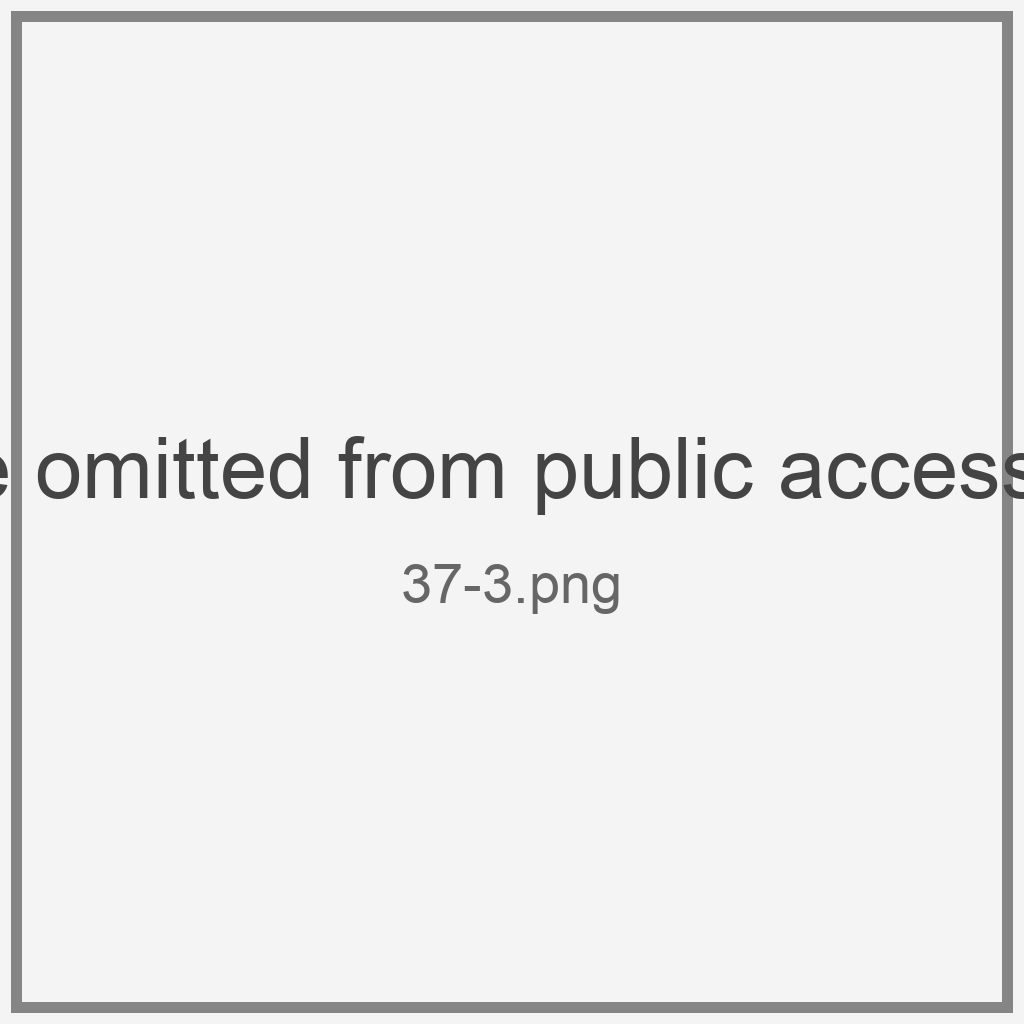
\includegraphics[width=0.52\textwidth]{Figures/rq3_cases/37-3.png}
    \caption[Image with the lowest participant set agreement.]{Image
    \texttt{37-3}, which had the lowest participant set agreement
    (\(J=.144\)). Harm was the most-endorsed category, selected by 5/16;
    GPT-5.6 and Qwen selected Harm, while GPT-4o selected Care. The woman's
    distress is clearly visible, while the social-media photograph leaves its
    cause open to interpretation.}
    \label{fig:rq3_37_3}
\end{figure}

The split has a plausible visual logic. The image makes the woman's distress
visible but leaves its cause unclear. Her tearful
expression, hand-to-head posture, discarded tissues, and disordered
surroundings make emotional distress the clearest cue. All three recorded
model explanations foregrounded these signs: GPT-5.6 and Qwen treated the
visible suffering as Harm, whereas GPT-4o framed the same vulnerability as a
need for Care. The phone introduces a less certain relational cue. Its screen
shows a social-media photograph of several smiling people together, but does
not establish who they are or why the woman is upset. Some participants may
therefore have inferred exclusion, rejection, or a breach of trust and
selected Betrayal. On this reading, Harm names the visible consequence, Care
the response that the woman's vulnerability invites, and Betrayal a possible
cause; an inferred betrayal could itself produce emotional harm.
\textbf{The disagreement may therefore separate labels for what is visible
from labels for what viewers inferred had caused it.} This explanation remains
tentative because participants could select multiple categories and their
reasons were not collected. The case illustrates why disagreement in a
subjective task can contain information that a single aggregated label removes
\cite{davani2022dealing,uma2021disagreement}.

Against this variable participant reference,
Table~\ref{tab:human_support_summary} summarises how often participants
included each model's label, weighting either responses or images equally. A
plurality match asks whether that label was among the most-endorsed categories
for an image; the more permissive top-two comparison also includes categories
ranked second, retaining ties.

\begin{table}[!htbp]
    \centering
    \caption{Participant inclusion of each model-selected category on the
    16-image survey subset. Intervals are descriptive 95\% bootstrap
    intervals.}
    \label{tab:human_support_summary}
    \footnotesize
    \setlength{\tabcolsep}{4pt}
    \begin{tabular}{lcccc}
        \toprule
        Model & \shortstack{Response-weighted\\endorsement (\%)} &
        \shortstack{Image-weighted\\endorsement (\%)} &
        \shortstack{Plurality\\set} &
        \shortstack{Top-two\\set} \\
        \midrule
        GPT-4o & 41.4 [36.1, 46.8] & 41.1 [29.6, 53.7] &
        9/16 (56.3\%) & 12/16 (75.0\%) \\
        GPT-5.6 & 47.9 [42.1, 53.6] & 47.5 [38.0, 58.1] &
        13/16 (81.3\%) & 15/16 (93.8\%) \\
        Qwen3.6 Flash & 40.7 [34.6, 46.8] & 40.4 [30.8, 50.0] &
        12/16 (75.0\%) & 13/16 (81.3\%) \\
        \bottomrule
    \end{tabular}
\end{table}

Across the 280 image--participant responses, the label that GPT-5.6 assigned
to each image was also selected by the participant in 134 cases (47.9\%). When
each of the 16 images was given equal weight, the corresponding rate was
47.5\%, showing that small differences in how many participants saw each image
did not drive the result. GPT-5.6's label was also among the most-endorsed
categories on 13 of the 16 images and among the top two on 15.
\textbf{Within this 16-image subset, GPT-5.6's labels corresponded most closely
with participant selections across all four summary measures.}

This is a narrower finding than saying that GPT-5.6 was generally closest to
human moral judgement. All three models returned the same label on ten of the
16 images, giving them identical participant endorsement on those cases. The
differences therefore came entirely from the other six images. Among these six,
GPT-5.6 selected a most-endorsed category on five, Qwen on four, and GPT-4o on
one. \textbf{GPT-5.6's lead was therefore produced by better correspondence on
a small set of model-disagreement cases, not by a broad difference across all
16 images.} GPT-5.6 ranked first on the reported summaries, but the ordering of
GPT-4o and Qwen changed with the measure: GPT-4o had slightly higher average
endorsement, whereas Qwen entered the most-endorsed set on more images. The
result should therefore be interpreted as a subset-specific comparison, not a
general model ranking. Complete image-level results are reported in Appendix
Table~\ref{tab:image_level_support}.

\FloatBarrier
\subsection{Consensus and Confidence Did Not Guarantee Participant Support}

Two images reveal opposite ways in which model and participant agreement came
apart. In image \texttt{o-1} (Figure~\ref{fig:rq3_o_1}), all 16 participants
endorsed Cheating, as did GPT-4o and GPT-5.6. Qwen instead selected
\textit{None} with confidence 95. Its recorded reason stated that there was no
visible looking or copying cue, although the man's gaze is directed towards the
other student's paper. At the output level, Qwen's scene description therefore
omitted a visible cue cited by the other two models. The difference may reflect
visual reading or the evidentiary threshold; it is not, by itself, evidence of
a different moral value.

Image \texttt{35-3} (Figure~\ref{fig:rq3_35_3}) shows the reverse pattern. All
three models selected \textit{None} with confidence between 91 and 95, but only
two of 18 participants endorsed \textit{None}; Loyalty was selected by 11.
All three recorded reasons identified a wedding celebration. GPT-5.6 and
Qwen even mentioned loyalty or social bonds as plausible associations, but
treated an ordinary celebration without a visible conflict as insufficiently
moral. One plausible explanation is the difference between instruments: the
participant definition linked Loyalty directly to commitment towards family
or a group, whereas the model prompt provided fuller decision guidance and an
explicit rule against unsupported moral inference
(Table~\ref{tab:instrument_comparison}). \textbf{The mismatch therefore appears
to concern the boundary of moral relevance rather than simple scene
recognition: most participants treated commitment itself as morally
meaningful, while all three models recognised the wedding but confidently
withheld a moral label.} The design cannot determine whether this boundary
difference came from task wording, response format, or a different threshold
for treating a scene as morally significant.

\textbf{Strong agreement within either group did not guarantee correspondence
between them.} Image \texttt{o-1} had a highly shared participant reading but
one model outlier;
image \texttt{35-3} had complete model agreement but little participant support
for the shared model label.

\begin{figure}[H]
    \centering
    \begin{subfigure}[t]{0.48\textwidth}
        \centering
        
\includegraphics[width=\textwidth,height=0.23\textheight,keepaspectratio]{Figures/rq3_cases/o-1.jpg}
        \caption{\texttt{o-1}: all 16 participants endorsed Cheating;
        Qwen selected \textit{None}.}
        \label{fig:rq3_o_1}
    \end{subfigure}
    \hfill
    \begin{subfigure}[t]{0.48\textwidth}
        \centering
        
\includegraphics[width=\textwidth,height=0.23\textheight,keepaspectratio]{Figures/rq3_cases/35-3.png}
        \caption{\texttt{35-3}: Loyalty received 11/18 endorsements;
        all three models selected \textit{None}.}
        \label{fig:rq3_35_3}
    \end{subfigure}
    \caption[Opposite separations between model and participant
    agreement.]{Opposite separations between model and participant agreement:
    a model outlier despite unanimous endorsement of one participant category
    (\texttt{o-1}), and unanimous model labels despite a different participant
    majority (\texttt{35-3}).}
    \label{fig:rq3_consensus_contrasts}
\end{figure}

Across the 16 images, the point estimates linking model-reported confidence to
participant endorsement were small
(Table~\ref{tab:confidence_endorsement}). Pearson correlations ranged from
.017 to .102 and rank correlations from .090 to .227. With only 16 selected
images and many tied confidence values, these estimates are too limited to
establish a general relationship.

\begin{table}[!htbp]
    \centering
    \caption{Association between model-reported confidence and participant
    endorsement of the selected category across the 16 survey images.}
    \label{tab:confidence_endorsement}
    \small
    \begin{tabular}{lcc}
        \toprule
        Model & Pearson \(r\) & Spearman \(\rho\) \\
        \midrule
        GPT-4o & .017 & .090 \\
        GPT-5.6 & .091 & .157 \\
        Qwen3.6 Flash & .102 & .227 \\
        \bottomrule
    \end{tabular}
\end{table}

The two illustrated cases make the limitation more concrete: Qwen reported
confidence 95 for the \textit{None} label that no participant selected on
\texttt{o-1}, and all three models reported 91--95 for the \textit{None} label
selected by only two participants on \texttt{35-3}. \textbf{Reported confidence
expressed the model's stated certainty within its task; in this subset, it did
not indicate how widely that interpretation was shared by participants.}

These comparisons measure correspondence with this participant sample, not
accuracy: participants could select several labels, whereas each model had to
return one. Removing only the \textit{None} selection from the three responses
in which it accompanied a moral category did not change any reported
model-label endorsement rate or participant plurality set, so these three
mixed responses did not drive the findings.

\textbf{RQ3 therefore separates three signals that should not be collapsed:
variation among participants, correspondence between a model label and those
participants, and the model's own confidence.} A model could match the leading
category when participant views were dispersed, models could agree on a label
that few participants selected, and high confidence could accompany either
pattern.

\paragraph{Supplementary Part~2.}
This exploratory survey component was not used to answer RQ1--RQ4. Its
item-level descriptive results are retained in
Appendix~\ref{app:part2_results}.


\FloatBarrier
\section{RQ4: Removing a Cue Was Not the Same as Reversing It}
\label{sec:rq4_results}

The 11 edited variants produced 33 attempted evaluations. One Qwen request
ended in a provider content-inspection error, leaving 32 valid base--variant
comparisons. Eight changed label: two of 11 for GPT-4o, three of 11 for
GPT-5.6, and three of ten for Qwen3.6 Flash. Those changes were not evenly
spread. Six variants left every available label unchanged, while five produced
at least one change. More strikingly, five of the eight label changes came from
only two edits: changing a distressed interaction to show positive expressions
and replacing a disaster setting with a peaceful one. \textbf{The most
revealing result was therefore not the overall change count, but the contrast
between removing information and giving the scene a different meaning.}

\subsection{The First Cue Removal Left Harm Intact}

Image \texttt{16-2} provided the clearest experimental sequence. All three
models initially selected Harm, and every primary explanation mentioned both
the restraint-like pose and visible pain or distress. Facial affect was
therefore a plausible candidate cue: if the Harm reading depended substantially
on it, obscuring the faces should at least weaken that reading and might change
the label. This was a working expectation in the exploratory sequence, not a
preregistered hypothesis.

The first edit obscured both faces while leaving the arm-around-neck pose
visible (Figure~\ref{fig:rq4_expression_sequence}). It did not change a single
label. GPT-4o remained at Harm 90; GPT-5.6 remained at Harm but fell from 96 to
82 confidence; and Qwen remained at Harm but fell from 95 to 85. The new
explanations focused on the restraint or chokehold-like body configuration.
The confidence reductions suggest that facial information strengthened the
judgement for two configurations, although all three still returned Harm
without it.

\begin{figure}[H]
    \centering
    \begin{subfigure}[t]{0.31\textwidth}
        \centering
        
\includegraphics[width=\linewidth,height=0.20\textheight,keepaspectratio]
        {Figures/rq4_cases/16-2_original.png}
        \caption{Original: Harm/Harm/Harm.}
    \end{subfigure}
    \hfill
    \begin{subfigure}[t]{0.31\textwidth}
        \centering
        
\includegraphics[width=\linewidth,height=0.20\textheight,keepaspectratio]
        {Figures/rq4_cases/16-2_faces_occluded.jpg}
        \caption{Faces obscured: Harm/Harm/Harm.}
    \end{subfigure}
    \hfill
    \begin{subfigure}[t]{0.31\textwidth}
        \centering
        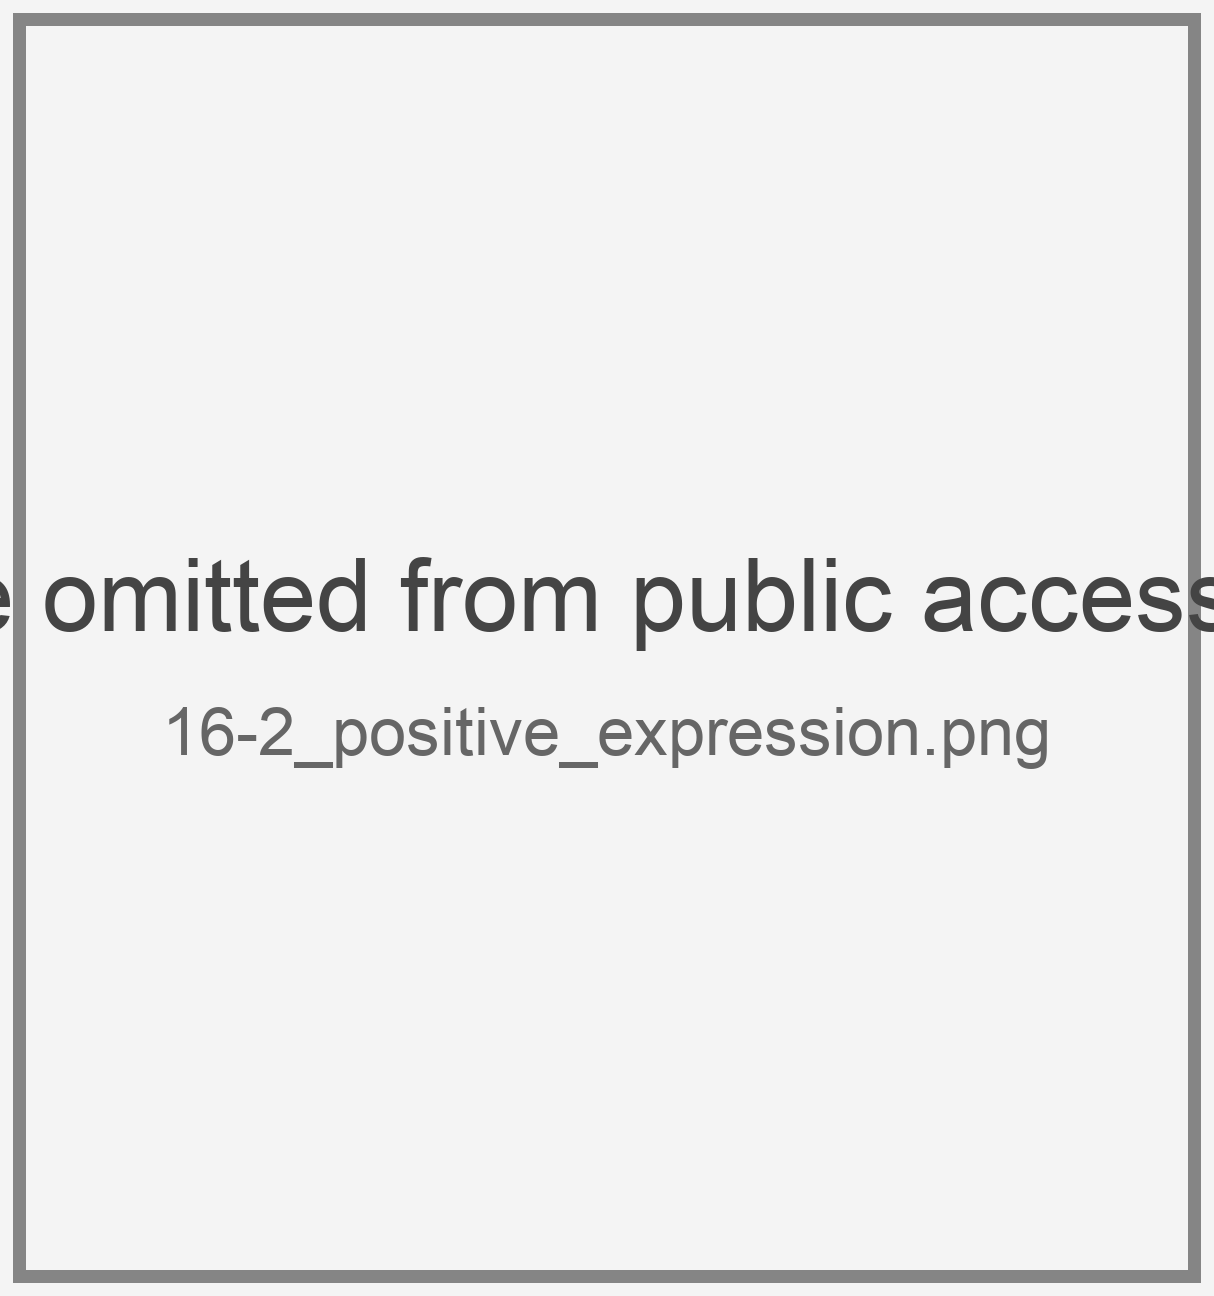
\includegraphics[width=\linewidth,height=0.20\textheight,keepaspectratio]
        {Figures/rq4_cases/16-2_positive_expression.png}
        \caption{Positive expressions: None/Loyalty/Care.}
    \end{subfigure}
    \caption[Sequential edits to facial information in image
    \texttt{16-2}.]{Sequential edits to facial information in image
    \texttt{16-2}. Labels are ordered as GPT-4o/GPT-5.6/Qwen3.6 Flash. Hiding
    the faces preserved Harm for all three models; changing the expressions
    was followed by three different alternatives.}
    \label{fig:rq4_expression_sequence}
\end{figure}

The follow-up edit did something different: it supplied positive expressions
while retaining the broad physical pose. This time every model left Harm, but
they did not converge on a new interpretation. GPT-4o selected \textit{None}
(85) and described playful contact without a clear moral concern. GPT-5.6
selected Loyalty (72), emphasising companionship and solidarity. Qwen selected
Care (85), emphasising affection and mutual well-being. \textbf{The models
agreed about what the image was no longer, but not about what it had become.}

A plausible explanation is that facial affect did not behave as a stand-alone
label trigger in this case. When facial information was absent, the visible
pose could still support an aggressive reading. When smiles contradicted that
reading, the same broad pose could instead appear playful or affectionate.
\textbf{In this case, missing facial evidence and facial evidence pointing in
the opposite direction were not equivalent.} The result concerns the relation
between cues, rather than a simple rule such as ``distress means Harm'' or
``smiling means Care.''

\subsection{Removing a Shared Context Exposed Different Readings}

Image \texttt{32-2} began with equally strong agreement: all three models
selected Harm, and their explanations centred on fire, smoke, destruction, and
danger. Replacing that disaster setting with a peaceful background tested
whether the common label would survive when the clearest environmental cue was
removed (Figure~\ref{fig:rq4_background_sequence}). The edit retained a closely
matched central figure, but foreground details, lighting, and framing also
changed; it was therefore not a background-only intervention.

\begin{figure}[H]
    \centering
    \begin{subfigure}[t]{0.46\textwidth}
        \centering
        
\includegraphics[width=\linewidth,height=0.25\textheight,keepaspectratio]
        {Figures/rq4_cases/32-2_original.png}
        \caption{Disaster setting: Harm/Harm/Harm.}
    \end{subfigure}
    \hfill
    \begin{subfigure}[t]{0.46\textwidth}
        \centering
        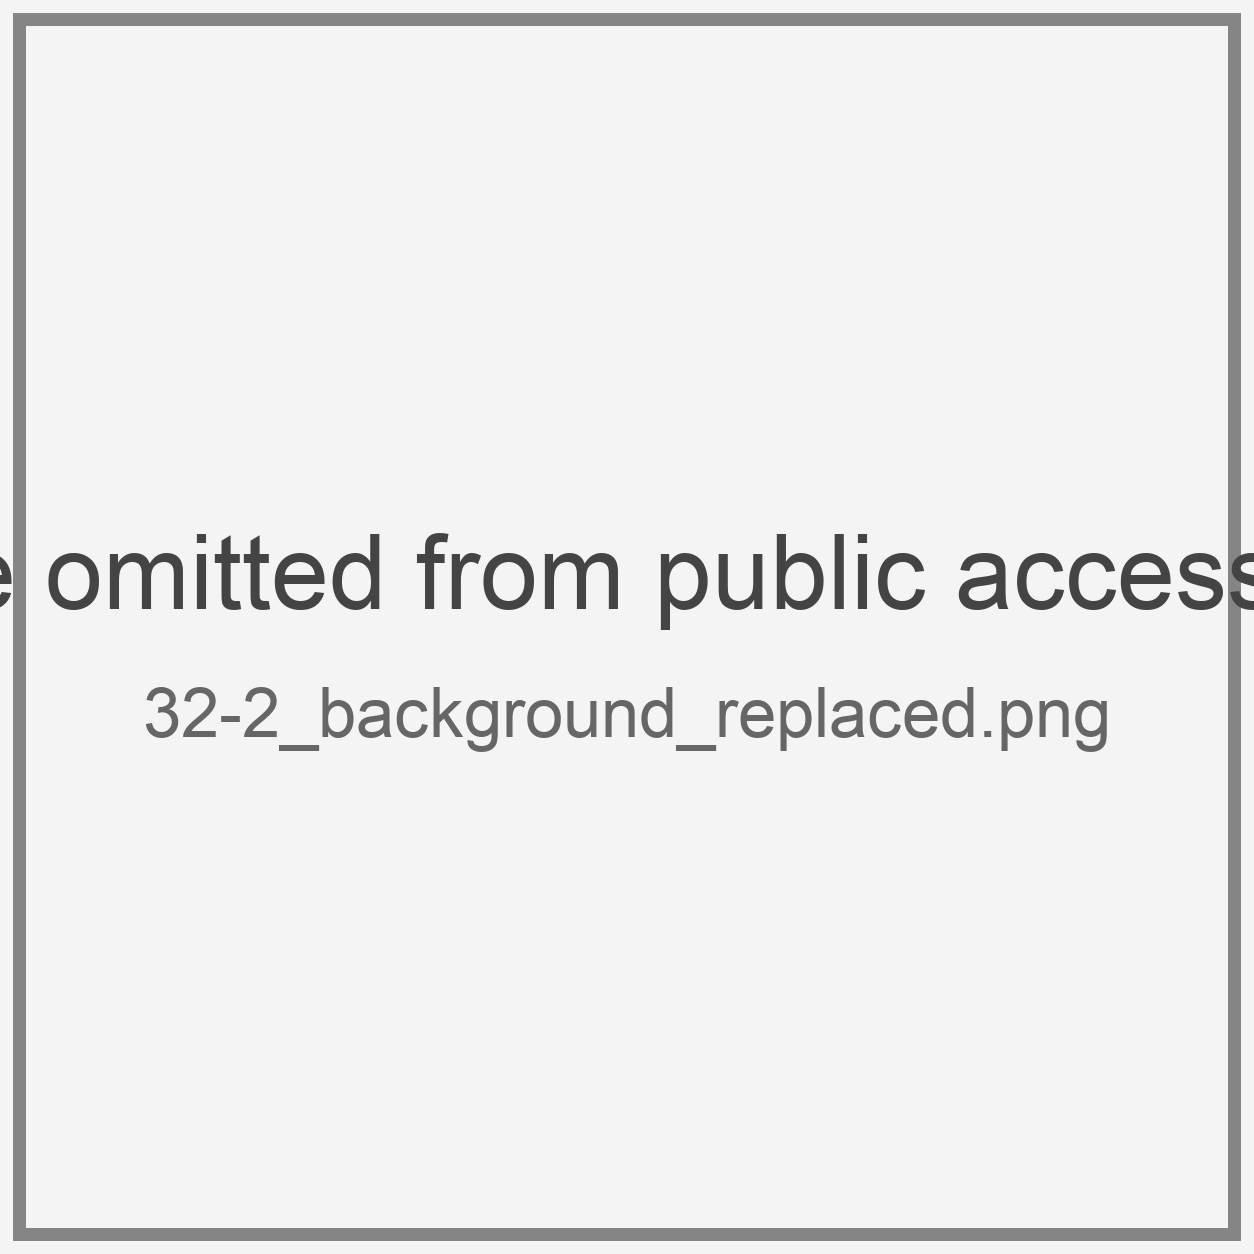
\includegraphics[width=\linewidth,height=0.25\textheight,keepaspectratio]
        {Figures/rq4_cases/32-2_background_replaced.png}
        \caption{Peaceful setting: Care/None/Harm.}
    \end{subfigure}
    \caption[Background replacement for image \texttt{32-2}.]{Background
    replacement for image \texttt{32-2}. Labels are ordered as
    GPT-4o/GPT-5.6/Qwen3.6 Flash. Removing the visible disaster was followed by
    three different readings of a similarly depicted central figure.}
    \label{fig:rq4_background_sequence}
\end{figure}

The expectation was only partly supported. GPT-4o changed from Harm 90 to Care
85, and its reason framed the edited figure's appearance as vulnerability.
GPT-5.6 changed from Harm 93 to \textit{None} 68; its reason said that no clear
moral event was visible. Qwen retained Harm, although its confidence fell from
95 to 75; its explanation treated the person's stained clothing and dishevelled
appearance as evidence of adversity. \textbf{Once the obvious danger cue was
removed, the models did not converge on neutrality. The edited foreground was
read as vulnerability, insufficient moral evidence, or continuing harm.}

This case helps explain a pattern seen in RQ2: agreement on a final label need
not mean that the models would draw the same moral boundary when a dominant cue
is weakened. The pair is consistent with the disaster context contributing to
the initial consensus; after the edited scene weakened that context, the
outputs diverged.

The two illustrated sequences contain five of the eight label changes, but
Table~\ref{tab:variant_transitions} records all 11 variants. Among the 24
comparisons in which the label stayed the same, reported confidence decreased
in 12, was unchanged in nine, and increased in three. A stable label therefore
did not always mean that an edit was irrelevant: it could weaken the reported
support without moving the answer across a category boundary. Mean confidence
changes were \(-1.82\) points for GPT-4o, \(-10.09\) for GPT-5.6, and
\(-4.00\) for Qwen,
but these provider-specific reports are not calibrated probabilities and
should not be compared as a common scale.

\begin{table}[p]
    \centering
    \caption{Complete base-to-variant record for the 11 edited variants.
    Authority abbreviates Respect/Authority; parentheses give the change in
    model-reported confidence in score points.}
    \label{tab:variant_transitions}
    \footnotesize
    \begin{spacing}{1.0}
    \setlength{\tabcolsep}{4pt}
    \renewcommand{\arraystretch}{1.08}
    \begin{tabularx}{\textwidth}{@{}L{0.18\textwidth}YYY@{}}
        \toprule
        Variant & GPT-4o & GPT-5.6 & Qwen3.6 Flash \\
        \midrule
        \texttt{16-1}, face occluded &
        Care 90 \(\rightarrow\) Care 85 (-5) &
        Care 94 \(\rightarrow\) Care 78 (-16) &
        Care 95 \(\rightarrow\) Care 95 (0) \\
        \addlinespace
        \texttt{16-2}, face occluded &
        Harm 90 \(\rightarrow\) Harm 90 (0) &
        Harm 96 \(\rightarrow\) Harm 82 (-14) &
        Harm 95 \(\rightarrow\) Harm 85 (-10) \\
        \addlinespace
        \texttt{16-1}, distressed expression &
        Care 90 \(\rightarrow\) Care 90 (0) &
        Care 94 \(\rightarrow\) Care 95 (+1) &
        Provider failure \\
        \addlinespace
        \texttt{16-2}, positive expression &
        Harm 90 \(\rightarrow\) None 85 (-5) &
        Harm 96 \(\rightarrow\) Loyalty 72 (-24) &
        Harm 95 \(\rightarrow\) Care 85 (-10) \\
        \addlinespace
        \texttt{1-1}, faces pixelated &
        Care 90 \(\rightarrow\) Care 90 (0) &
        Care 96 \(\rightarrow\) Care 82 (-14) &
        Care 95 \(\rightarrow\) Care 95 (0) \\
        \addlinespace
        \texttt{1-1}, contact region occluded &
        Care 90 \(\rightarrow\) Care 95 (+5) &
        Care 96 \(\rightarrow\) Care 88 (-8) &
        Care 95 \(\rightarrow\) Care 95 (0) \\
        \addlinespace
        \texttt{7-2}, body/pose occluded &
        Authority 95 \(\rightarrow\) Authority 90 (-5) &
        Authority 92 \(\rightarrow\) Authority 92 (0) &
        Authority 95 \(\rightarrow\) Authority 85 (-10) \\
        \addlinespace
        \texttt{34-1}, text removed &
        Authority 85 \(\rightarrow\) Authority 85 (0) &
        Degradation 68 \(\rightarrow\) Authority 62 (-6) &
        Harm 85 \(\rightarrow\) Harm 75 (-10) \\
        \addlinespace[8pt]
        \texttt{g-7}, group region occluded &
        None 90 \(\rightarrow\) None 85 (-5) &
        Loyalty 78 \(\rightarrow\) Loyalty 66 (-12) &
        Care 75 \(\rightarrow\) None 95 (+20) \\
        \addlinespace
        \texttt{12-1}, hand/gesture occluded &
        Sanctity 85 \(\rightarrow\) Sanctity 85 (0) &
        Sanctity 78 \(\rightarrow\) Sanctity 85 (+7) &
        Sanctity 85 \(\rightarrow\) None 85 (0) \\
        \addlinespace
        \texttt{32-2}, background replaced &
        Harm 90 \(\rightarrow\) Care 85 (-5) &
        Harm 93 \(\rightarrow\) None 68 (-25) &
        Harm 95 \(\rightarrow\) Harm 75 (-20) \\
        \bottomrule
    \end{tabularx}
    \end{spacing}
\end{table}

The complete original--variant image set is reproduced in
Appendix~\ref{app:edit_images}. These cases relate to controlled evidence that VLM moral judgements can change
under visual perturbations \cite{liu2026moralbackbone}, but the present question
is narrower. Several edits here deliberately changed morally relevant content,
so a changed label is not automatically a robustness failure. The edits were
also not perfectly isolated: the expression and background variants changed
other image details, and the base and edited images were evaluated in different
inference blocks. The results therefore identify case-level associations, not
causal feature attributions or general provider rankings.

\textbf{RQ4's central finding is not simply that the outputs were fragile. In
these cases, removing a cue often left the original moral frame intact, whereas
supplying a conflicting expression or context could reorganise the moral
reading of the scene and reveal different alternatives across models.}

\FloatBarrier

\section{Exploratory Prompt-Robustness Check}
\label{sec:prompt_robustness_results}

The three prompt conditions are summarised in
Section~\ref{sec:prompt_robustness_design}, and the exact P1 and P2 additions
are reproduced in Appendix~\ref{app:repeat_prompt}. All 432 planned outputs
were obtained, but Table~\ref{tab:prompt_robustness} shows that the prompt
variants produced little change in the RQ3 participant comparison.

\begin{table}[H]
    \centering
    \caption{Image-weighted participant endorsement under the baseline (P0),
    structured (P1), and cue-guided (P2) prompts. Values are percentages; the
    final column reports the P2--P0 change in percentage points.}
    \label{tab:prompt_robustness}
    \small
    \begin{tabular}{lrrrr}
        \toprule
        Model & P0 & P1 & P2 & P2--P0 \\
        \midrule
        GPT-5.6       & 44.6\% & 43.6\% & 45.3\% & \(+0.7\) \\
        GPT-4o        & 41.5\% & 41.9\% & 41.1\% & \(-0.4\) \\
        Qwen3.6 Flash & 39.5\% & 40.1\% & 39.5\% & \(0.0\) \\
        \bottomrule
    \end{tabular}
\end{table}

For the primary GPT-5.6 comparison, the P2--P0 difference was small and
uncertain (95\% image-bootstrap interval: \(-1.0\) to 3.1; exact sign-flip
\(p=1.000\)). P0 and P2 also produced the same modal label on all 16 images and
the same 11/16 plurality matches. P1 and the other models likewise
showed only small, mixed changes, while GPT-5.6 retained the highest descriptive
correspondence under all three conditions. \textbf{The narrow robustness
finding is that the subset-specific ordering reported in RQ3 did not change;
cue guidance itself did not consistently improve participant correspondence.}
Because P0 used new repeated calls, its percentage differs from the single
retained output reported in RQ3. These results do not establish a general model
ranking.

\FloatBarrier

\section{What the Four Research Questions Reveal Together}
\label{sec:results_synthesis}

Across the four research questions, one story recurred: \textbf{the models did
not simply detect a moral category already present in an image; their outputs
reflected a moral reading built from visible evidence and contextual
assumptions.} RQ1 distinguished whether a scene was classified as morally
relevant from how its moral meaning was framed. RQ2 carried this story from
disagreement between models to variation within a model. The models more
readily shared the judgement that a scene was morally significant than the
moral reading used to explain it. Across evaluation windows, the same model
could return a different reading of the same image and then repeat that reading
across the later calls.

RQ3 found that participants also produced competing readings; even unanimous
model labels or high reported confidence could receive little participant
support. RQ4 showed how readings changed in the selected cases. Obscuring facial
information left the original label intact, whereas positive expressions or a
replaced disaster setting coincided with different interpretations across
models. These cases were consistent with models reading facial affect, body
pose, and scene context in combination, but the edits did not isolate the
effect of any one cue.

Taken together, the findings show that \textbf{apparent consensus can hide
different interpretive boundaries}. In the selected cases, models shared a
label before an edit but diverged after the relevant visual evidence was
changed. Model agreement, short-run repeatability, comparison with researcher
coding, participant endorsement, and reported confidence therefore describe
distinct properties of the outputs; none alone establishes which
interpretation is correct. Although the edits cannot isolate a causal feature, they show how one label
can conceal different readings of the same scene.

\FloatBarrier
